\documentclass{experimentreport}

\input{listing_style.tex}

\usepackage{amsmath}
\usepackage{booktabs}
\usepackage{caption}
\usepackage{enumitem}
\usepackage{float}
\usepackage{graphicx}
\usepackage{makecell}

\graphicspath{{../results/figures/}}
\captionsetup{font=small,labelfont=bf,labelsep=quad}
\setlist{nosep,leftmargin=2.2em}
\setlength{\emergencystretch}{2em}

%========================
% 基本信息
%========================

\setcoursename{基础软件开发技术实践}
\setreportname{智能软件工程实验报告}

\setexperimenttitle{实验六：改进针对大模型生成代码的代码审查}

\setstudentname{\hintholder{王皓}}
\setdepartment{\hintholder{计算学部}}
\setstudentid{\hintholder{2023111825}}

\setcourseteacher{刘佳琨}
\setinstructor{刘佳琨}

\setlablocation{\hintholder{格物213}}
\setlabtime{    \hintholder{2026年7月9日}}

\begin{document}

%========================
% 自动生成封面
%========================

\makereporthead

%========================
% 实验目的
%========================

\experimentpurpose{

完成本实验后，学生应能够：

\begin{enumerate}[label=\arabic*.]
	\item 理解 AI 生成代码代码审查性能下降的主要原因。
	\item 掌握不同代码上下文构建方法及其对代码审查任务的影响。
	\item 掌握 Prompt Engineering 优化代码审查性能的方法。
	\item 能够设计适用于 AI 生成代码的 Prompt。
	\item 能够分析不同 Prompt 和上下文组合对 Merge Prediction 和 Review Comment Generation 任务的影响。
	\item 能够提出针对 AI 生成代码的代码审查改进方案。
\end{enumerate}

}

%========================
% 实验内容
%========================

\experimentcontent{

\subsection{任务定义与技术路线}

实验五揭示了两项直接影响结论的问题。AI 分类样本中已合并 PR 占 74\%，近似恒预测“合并”仍可获得约 0.74 的 Accuracy 和 0.85 的 merge-F1，总体指标由此掩盖了未合并类的识别缺陷。开放式审查意见与单条参考意见的词面重合普遍较低，BLEU 和 ROUGE 难以反映意见的相关性、正确性和可执行性。实验四、五的 C1--C4 仅包含 diff 及 PR 文本等浅层信息，深层软件工程上下文的作用仍需检验。

本实验固定执行模型及其参数，通过上下文和 Prompt 两类输入变量回答三个问题：深层上下文能否改善分类判别力和审查意见质量；Self-Reflection 与多轮交互如何影响默认合并偏向；质量变化与额外时延之间存在何种权衡。匹配人类代码对照进一步检验输入方案对不同代码来源的适用性。整体流程为

\begin{center}
\fbox{\parbox{0.93\textwidth}{
\centering
实验五固定 AI 样本
$\longrightarrow$ L0--L4 单调上下文阶梯
$\longrightarrow$ P*、P5、P6 Prompt
$\longrightarrow$ \texttt{deepseek-v4-flash} 推理
$\longrightarrow$
\begin{tabular}{c}
Merge Prediction\\
Review Comment Generation
\end{tabular}
$\longrightarrow$ 分类逐类评估、生成多维裁判、消融与人类对照
}}
\end{center}

评价设计先建立能够反映真实错误分布的测量指标，再用上下文阶梯和 Prompt 消融定位性能变化的来源。分类任务报告 balanced accuracy、逐类 Precision/Recall 和混淆矩阵；生成任务由 \texttt{deepseek-v4-pro} 从四个维度评价意见质量。两类指标与推理时延共同构成实验的证据链。

\subsection{数据来源与实验矩阵}

数据直接取自实验五的固定样本。Merge Prediction 使用 50 个 AI PR，其中 37 个已合并、13 个未合并；Review Comment Generation 使用 72 个至少包含一条顶层行内审查意见的 AI PR。生成真值沿用实验四、五的统一口径，每个 PR 取时间最早的非回复顶层 inline comment。人类对照沿用实验五的 \texttt{matched\_human\_control}，从实验二 held-out test 中按 AI 样本的仓库与合并标签分布匹配抽取。

实验矩阵围绕上下文、Prompt、二者归因和代码来源四项比较展开（表~\ref{tab:exp-matrix}），每项任务包含 10 个去重条件。旧最优 Prompt P* 在实验六运行前由实验五 AI 结果确定：分类选择跨上下文平均 Accuracy 最高的 P1（0.760），生成选择按原评价口径平均 BLEU 最高的 P3（1.125）。这一预选结果作为上下文阶梯和新 Prompt 的统一比较基线。

\begin{table}[H]
\centering
\caption{实验六的假设驱动实验矩阵。P* 为实验五数据上预先选定的旧最优 Prompt；人类对照仅运行关键条件，以控制调用成本。}
\label{tab:exp-matrix}
\small
\begin{tabular}{lll}
\toprule
分析目的 & AI 代码条件 & 人类对照条件 \\
\midrule
上下文消融 & $\{\mathrm{L0,L1,L2,L3,L4}\}\times\mathrm{P*}$ & -- \\
Prompt 消融 & $\mathrm{L4}\times\{\mathrm{P*,P5,P6}\}$ & -- \\
作用归因 & $\mathrm{L0}\times\mathrm{P5}$ & -- \\
来源泛化 & -- & $\mathrm{L4}\times\{\mathrm{P*,P5}\}$ \\
\bottomrule
\end{tabular}
\end{table}

\subsection{单调递增的软件工程上下文}

上下文模块实现统一接口 \texttt{build\_context(repo, number, level)}，构造 L0--L4 五级单调阶梯（表~\ref{tab:context-levels}）。L0 与实验四 C1 完全一致，仅拼接 PR 内 Python 文件的 patch；L1 对应实验四 C4，加入 PR 标题、正文及全部 Commit Message；L2 依据 base SHA 和 head SHA 拉取修改前后的文件，并优先抽取改动 hunk 所在的完整函数或类；L3 从 PR 正文解析 Issue 引用，加入 Issue 标题、正文和历史 review/comment；L4 再对被改符号执行仓库内轻量词法检索，并补充同目录文件头和仓库贡献约定。L3 构建生成输入时显式排除作为真值的目标评论，防止标签泄漏。

\begin{table}[H]
\centering
\caption{L0--L4 上下文构建样例与实测规模。每一级保留低级信息并新增一种工程证据；字符数为 50 个 AI 分类样本的平均值。}
\label{tab:context-levels}
\small
\begin{tabular}{cllr}
\toprule
级别 & 新增证据 & 输出中的典型标记 & 平均字符数 \\
\midrule
L0 & Python Diff & 文件路径与 patch & 5,916 \\
L1 & PR 描述、全部 Commit Message & \texttt{PR 描述}、\texttt{Commit 信息} & 8,164 \\
L2 & 改前/改后完整函数或文件 & \texttt{改前/改后完整函数 (L2)} & 30,019 \\
L3 & Issue 正文、历史审查意见 & \texttt{关联 Issue 与历史审查 (L3)} & 32,464 \\
L4 & 符号检索、同目录文件头、仓库约定 & \texttt{仓库级检索上下文 (L4)} & 35,205 \\
\bottomrule
\end{tabular}
\end{table}

各层采用独立字符预算和固定优先级截断。Diff、PR 正文和 Commit Message 沿用实验四预算；L2 分别限制单文件代码和全部文件的长度；L3 分别限制 Issue 与历史审查长度；L4 限制检索符号数、每个符号的 top-$k$ 文件数和单片段长度。GitHub API 返回的文件、Issue 与检索结果按请求键落盘缓存。L4 采用轻量词法检索，动态获取符号出现位置、同目录文件头和仓库约定，用于测量仓库级词法证据的边际作用。

\subsection{Prompt 设计与模型推理}

旧 Prompt P1--P4 分别为 Zero-shot、Few-shot、Chain-of-Thought（CoT）和 Role-based。P5 Self-Reflection 通过两阶段顺序引导审查：第一阶段以 maintainer 角色主动列出 blocking defects，第二阶段根据缺陷清单给出结论。分类任务输出 \texttt{blocking\_defects + reasoning + decision} 结构化 JSON，标签为 \texttt{MERGE} 或 \texttt{REJECT}；生成任务在第二阶段输出具体、可操作的行内意见。P6 则将反思过程展开为多轮交互。

\begin{table}[H]
\centering
\caption{P5 Self-Reflection 的核心 Prompt 样例。结构化阶段约束用于改变审查姿态，同时保持与已有输出解析器兼容。}
\label{tab:p5-sample}
\small
\begin{tabular}{p{0.14\textwidth}p{0.76\textwidth}}
\toprule
阶段 & 指令摘要 \\
\midrule
阶段 1 & 以挑剔 maintainer 视角主动寻找所有 blocking 缺陷；不预设 PR 正确，若确无缺陷则明确记录。 \\
阶段 2 & 基于阻断性缺陷清单复核证据；存在任一 blocking 缺陷时倾向拒绝，否则才判定合并。 \\
输出约束 & 分类返回缺陷、推理和 \texttt{decision}；生成返回与代码位置和修改动作对应的 \texttt{comment}。 \\
\bottomrule
\end{tabular}
\end{table}

P6 将分类拆为“描述改动--追问遗漏风险--最终判定”三轮，将生成拆为“意见初稿--自我批评--修订意见”三轮。每轮把上一轮 assistant 回复加入消息历史，并形成独立缓存键。P6 的三次调用成本较高，实验将其安排在信息最完整的 L4 条件。执行模型统一使用 \texttt{deepseek-v4-flash}，分类温度为 0，生成温度为 0.3，模型权重保持固定。语义缓存的内容哈希包含实际模型标识、messages、温度和最大输出长度，执行结果与裁判结果使用不同缓存键。

\subsection{评价指标与结果分析设计}

对于 Merge Prediction，设未合并类和已合并类的召回率分别为 $R_{\mathrm{nm}}$ 与 $R_{\mathrm{m}}$，主指标 balanced accuracy 定义为
\[
\mathrm{BAcc}=\frac{R_{\mathrm{nm}}+R_{\mathrm{m}}}{2}.
\]
实验还报告两类 Precision、Recall、F1 及混淆矩阵中的 TN、FP、FN、TP。Balanced accuracy 和 non-merge recall 用于判断分类改进，Accuracy 和 merge-F1 用于复现实验五口径。

对于 Review Comment Generation，裁判模型 \texttt{deepseek-v4-pro} 接收生成意见、参考意见和 Diff，从 relevance、actionable、correct、hallucination 四个维度给出 1--5 分及理由，其中前三项越高越好，hallucination 越低越好。综合质量分将 hallucination 转换为 $6-\mathrm{hallucination}$ 后与其余三维等权平均。BLEU 与 ROUGE-1/2/L 复现实验五的词面评价口径。

结果分析依次执行四类比较：上下文阶梯定位有效证据层；L4 Prompt 消融检验推理姿态；L0$\times$P5、L4$\times$P* 与 L4$\times$P5 共同区分 Prompt 和上下文的作用；匹配人类对照检验来源泛化。分类错误转移使用同一批 50 个 PR 逐样本配对；图中不确定性采用固定随机种子、2,000 次 bootstrap 得到 95\% 置信区间。每个条件同时记录推理时延，以支持质量--成本权衡。

\subsection{实现架构与可复现性}

实验使用 Python~3.12 与 \texttt{uv} 管理环境。\texttt{data.py} 读取实验五固定样本并连接实验一数据表，\texttt{github\_fetch.py} 负责限流、重试和 API 缓存，\texttt{context\_builder.py} 构建 L0--L4，\texttt{prompts.py} 定义 P5/P6，\texttt{run\_experiments.py} 编排矩阵，\texttt{judge.py} 完成生成裁判，\texttt{evaluate.py} 汇总指标，\texttt{nature\_viz.py} 导出图件及 source CSV。逐样本预测保存为 Parquet，汇总指标保存为 JSON；图件同时导出 SVG、PDF 和 600~dpi PNG。固定样本、确定性截断、API/LLM 双缓存和图件源数据共同保证实验可复现，并为实验七 VSCode 插件中的分级审查策略提供下游依据。

}

%========================
% 实验结果
%========================

\experimentresult{

\subsection{总体结果：输入优化改变了错误分布}

图~\ref{fig:overview}概括了输入优化对两项任务的影响。L4 下，旧 Prompt 的 merge recall 接近饱和，non-merge recall 很低；P5 和 P6 提高了 non-merge recall，并降低了 merge recall。三种 Prompt 的生成复合质量接近。输入设计对分类错误分布的影响较强，对生成综合质量的影响较弱。

\begin{figure}[H]
\centering
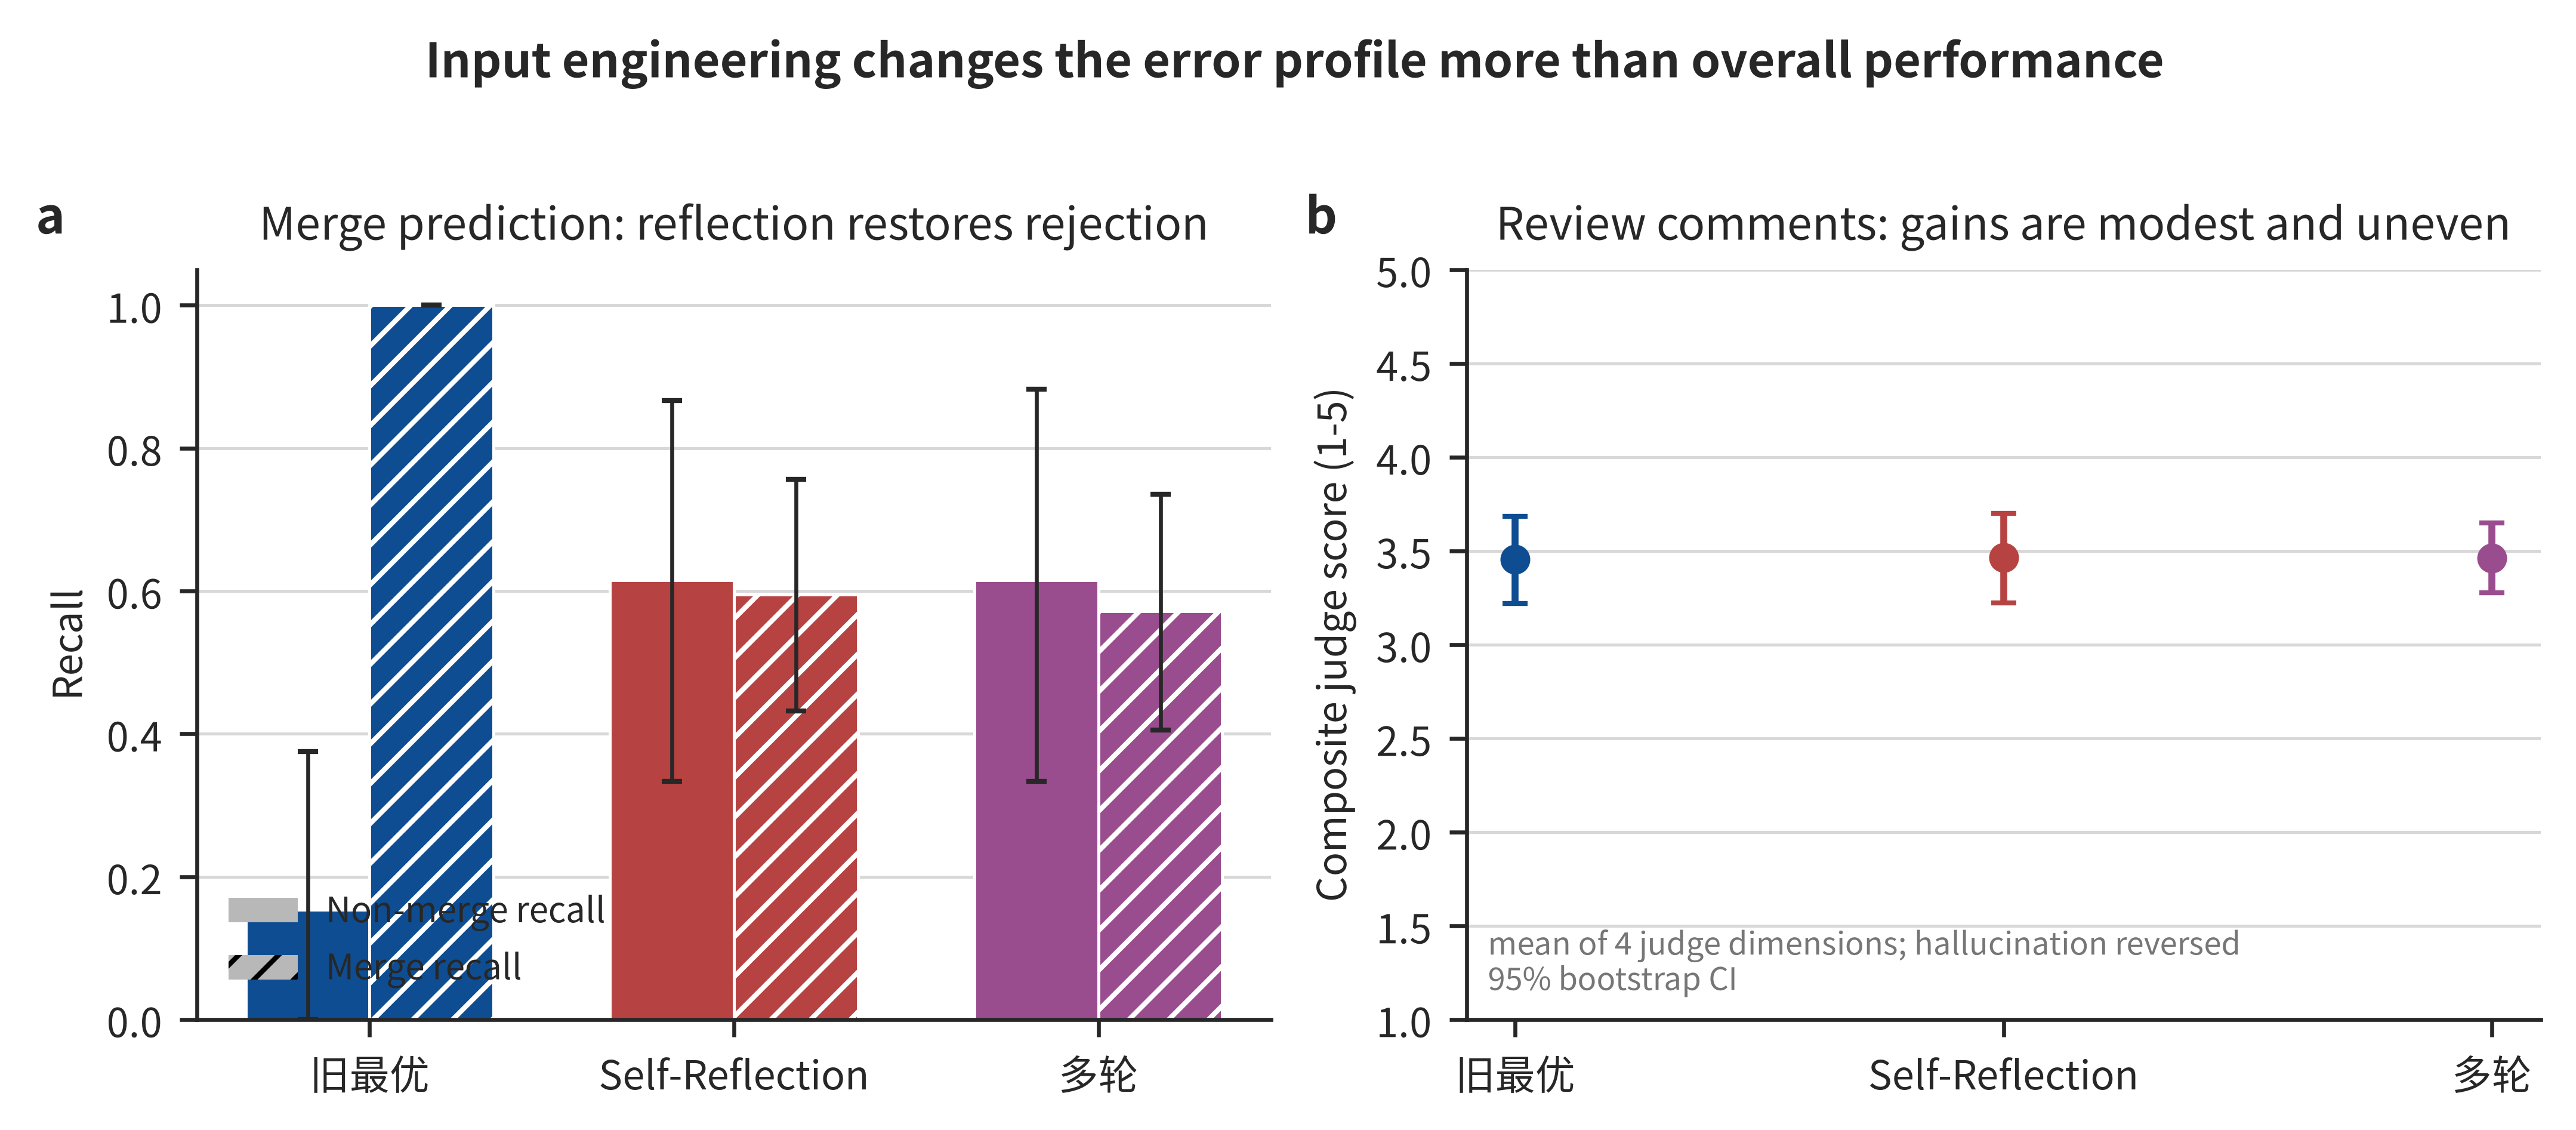
\includegraphics[width=0.98\textwidth]{fig1_result_overview.pdf}
\caption{实验六结果总览。\textbf{a}，L4 下三种 Prompt 对未合并类与已合并类的 Recall；分类每格 $n=50$。\textbf{b}，Review Comment Generation 的四维等权复合质量，其中 hallucination 以 $6-x$ 反向计分；生成每格 $n=72$。点为样本统计量，误差线为固定随机种子、2,000 次 bootstrap 的 95\% 置信区间。输入优化主要移动分类决策工作点，三种 Prompt 的生成复合质量则高度接近。}
\label{fig:overview}
\end{figure}

在 L4 上，旧 P1 的 merge recall 为 1.000，13 个未合并 PR 中识别出 2 个。P5 将 non-merge recall 从 0.154 提高至 0.615，merge recall 降至 0.595。旧 P3、P5 和 P6 的生成复合质量分别为 3.454、3.465 和 3.462，最大差值为 0.011，置信区间高度重叠。P5 主要调整了分类工作点，三种 Prompt 的生成综合质量处于同一水平。

\subsection{上下文阶梯：相关性比长度更重要}

固定旧最优 Prompt 后，上下文阶梯呈现非单调变化（图~\ref{fig:context-ladder}）。分类从 L0 到 L2 的 balanced accuracy 由 0.538 升至 0.583，non-merge recall 由 0.077 升至 0.167，完整函数或文件补充了局部 patch 缺少的实现信息。L3 和 L4 的混淆矩阵相同，均为 TN=2、FP=11、FN=0、TP=37，balanced accuracy 为 0.577。各层置信区间覆盖或接近 0.5，L2 的较高点估计仍需更大样本验证。

\begin{figure}[H]
\centering
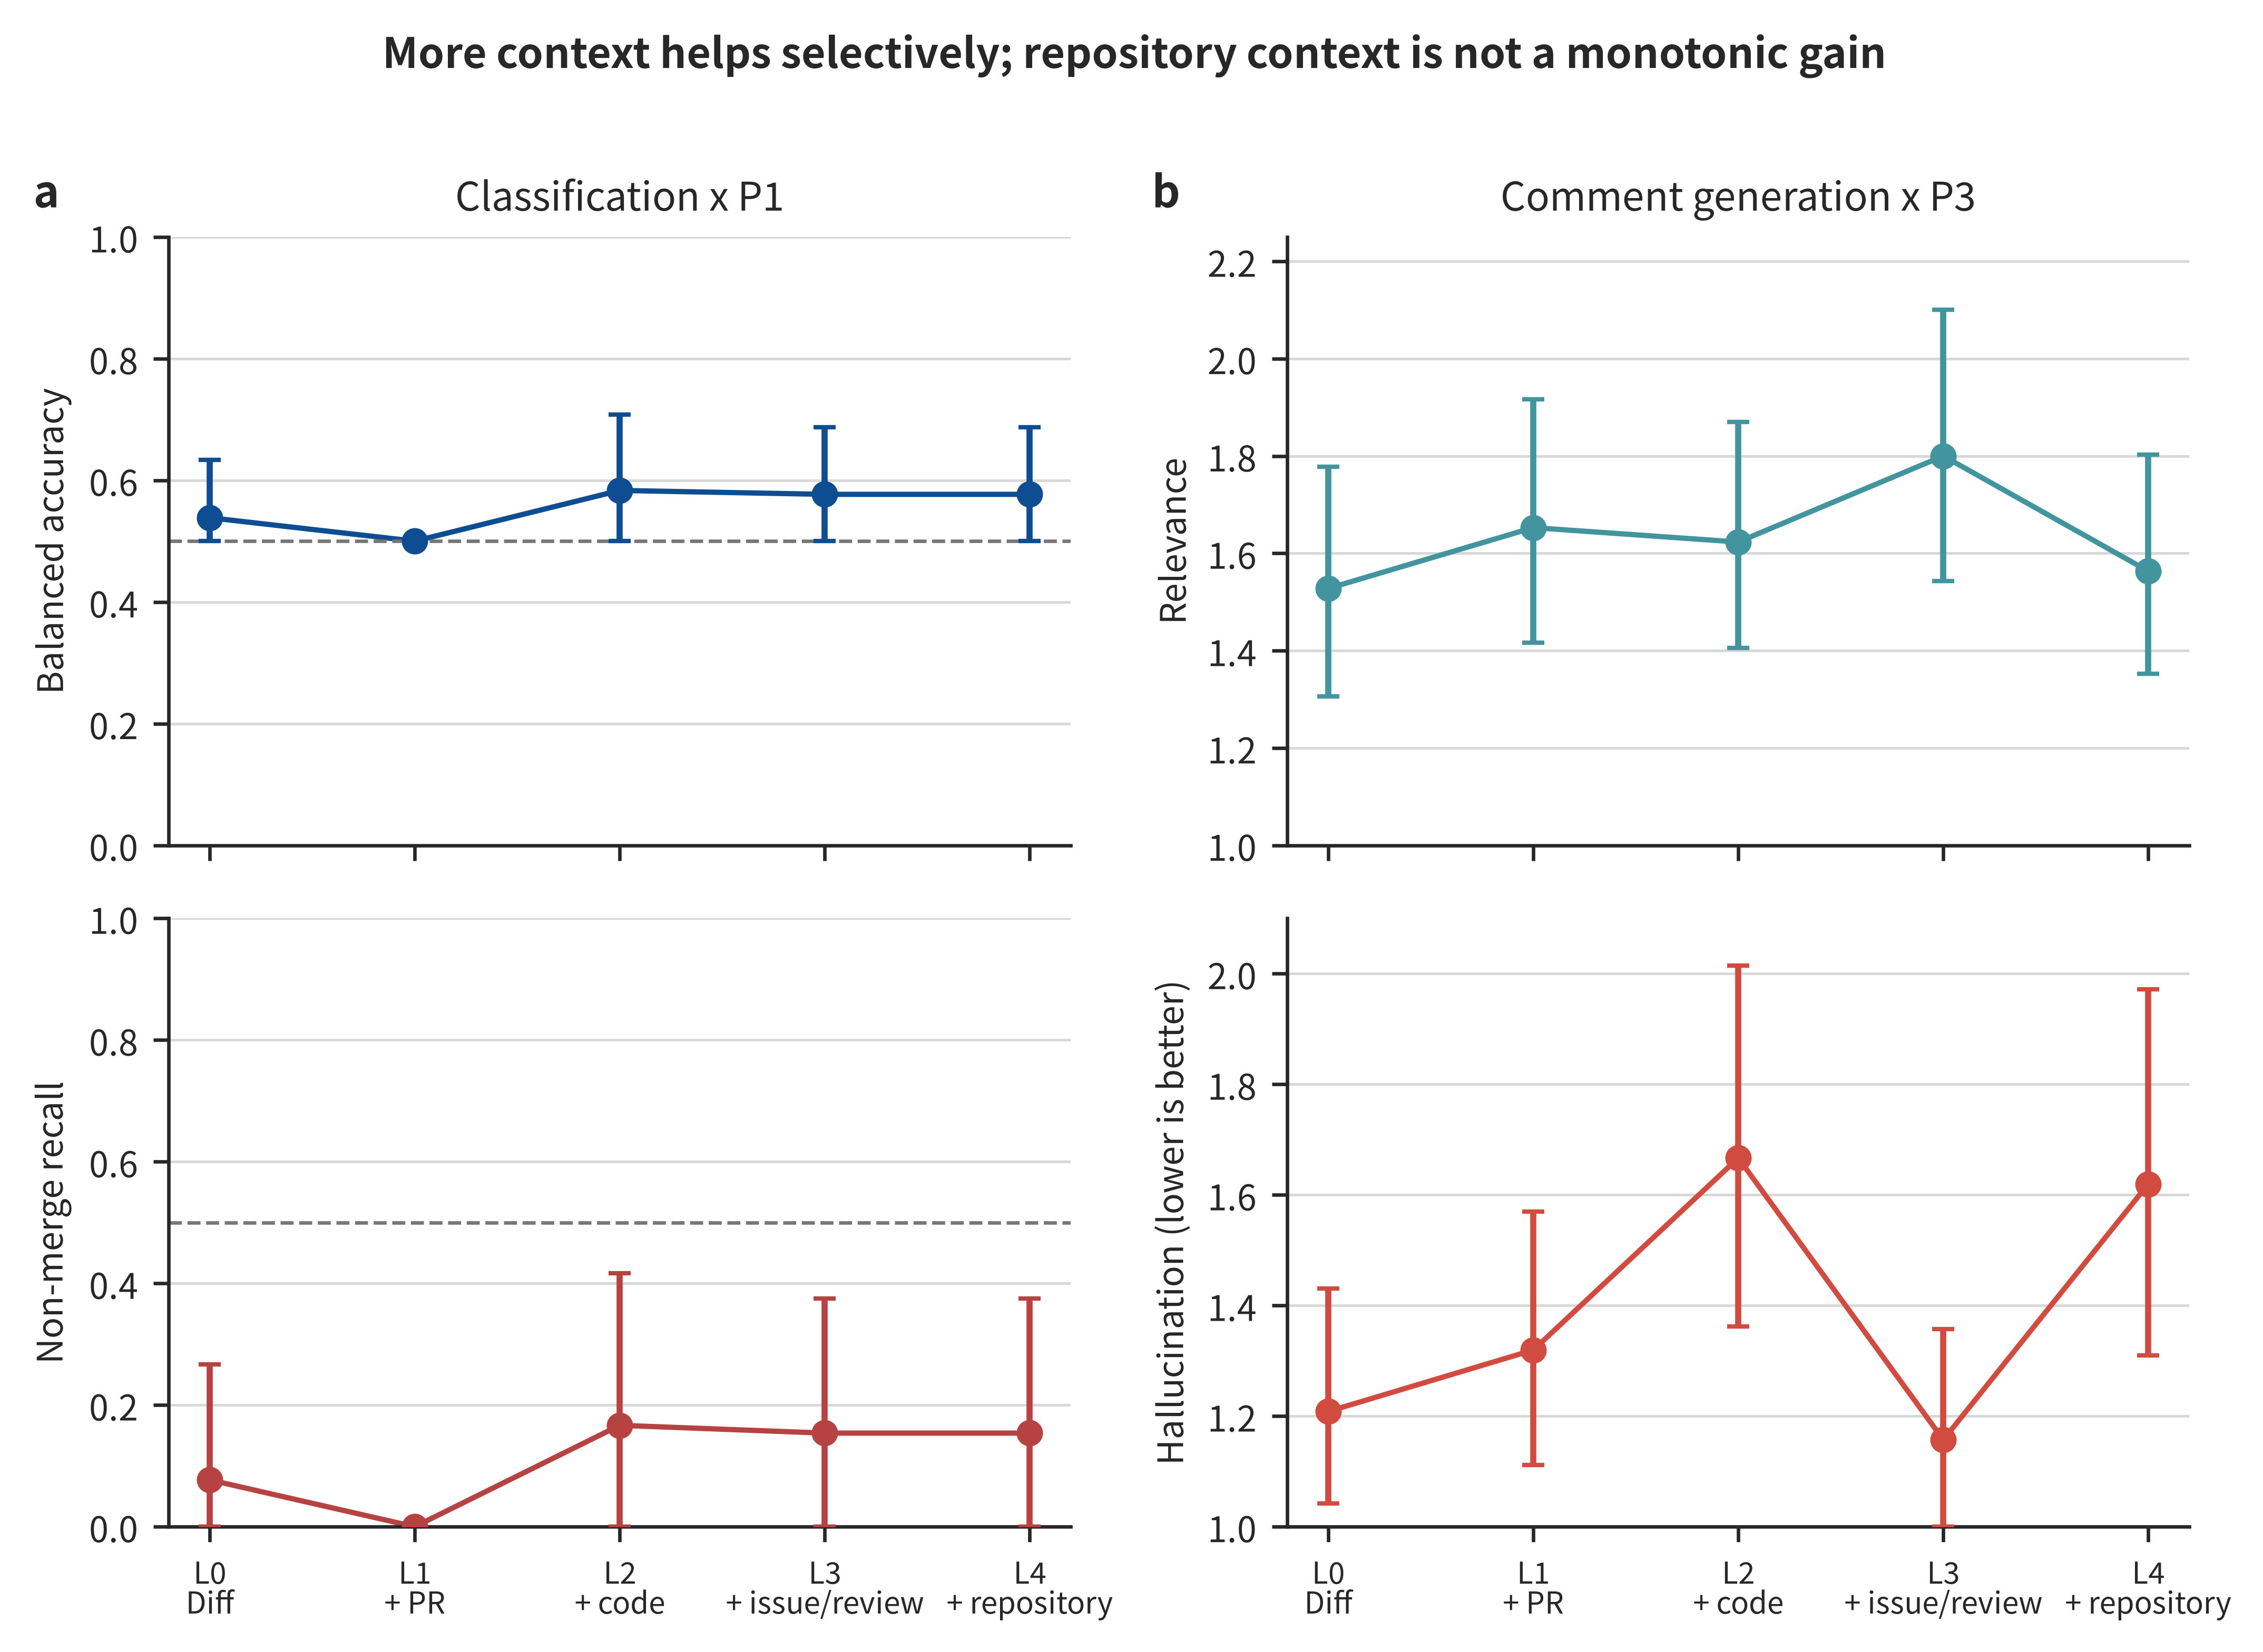
\includegraphics[width=0.98\textwidth]{fig2_context_ladder.pdf}
\caption{上下文阶梯的任务差异。\textbf{a}，P1 下 Merge Prediction 的 balanced accuracy 与 non-merge recall，虚线表示无判别基准 0.5。\textbf{b}，P3 下 Review Comment Generation 的 relevance 与 hallucination。点为样本统计量，误差线为 95\% bootstrap 置信区间。分类在 L2 获得有限点估计增益，生成在 L3 的四维质量最佳；继续加入 L4 词法片段并未带来单调改善。}
\label{fig:context-ladder}
\end{figure}

\begin{table}[H]
\centering
\caption{固定旧最优 Prompt 时的上下文阶梯结果。分类报告 balanced accuracy、Accuracy 及两类 Precision/Recall/F1；生成报告四维裁判分数，hallucination 越低越好。P/R/F1 三元组依次表示 Precision、Recall 和 F1。}
\label{tab:context-results}
\small
\resizebox{\textwidth}{!}{%
\begin{tabular}{lrrrrrrrr}
\toprule
条件 & BAcc & Accuracy & Non-merge P/R/F1 & Merge P/R/F1 & Relevance & Actionable & Correct & Hallucination$\downarrow$ \\
\midrule
L0$\times$P* & 0.538 & 0.760 & 1.000/0.077/0.143 & 0.755/1.000/0.860 & 1.528 & 3.736 & 3.917 & 1.208 \\
L1$\times$P* & 0.500 & 0.740 & 0.000/0.000/0.000 & 0.740/1.000/0.851 & 1.653 & 3.958 & 3.958 & 1.319 \\
L2$\times$P* & \textbf{0.583} & \textbf{0.796} & 1.000/0.167/0.286 & 0.787/1.000/\textbf{0.881} & 1.623 & 3.725 & 3.768 & 1.667 \\
L3$\times$P* & 0.577 & 0.780 & 1.000/0.154/0.267 & 0.771/1.000/0.871 & \textbf{1.800} & \textbf{4.229} & \textbf{4.214} & \textbf{1.157} \\
L4$\times$P* & 0.577 & 0.780 & 1.000/0.154/0.267 & 0.771/1.000/0.871 & 1.563 & 4.085 & 3.789 & 1.620 \\
\bottomrule
\end{tabular}
}
\end{table}

生成任务在 L3 获得最高 relevance（1.800）、actionable（4.229）、correct（4.214）和最低 hallucination（1.157）。Issue 需求与历史审查为意见生成提供了直接相关的任务信息。L4 的 BLEU 升至 2.259，relevance 降至 1.563，hallucination 升至 1.620。词面指标与四维质量给出了不同排序，说明上下文选择应优先关注任务相关性。L3 与 L4 的 relevance 置信区间仍有重叠，两层差异属于候选趋势。

\subsection{Prompt 消融：Self-Reflection 移动分类工作点}

L4 下的 Prompt 消融结果见表~\ref{tab:prompt-results} 与图~\ref{fig:prompt-tradeoff}。P5 和 P6 均将 non-merge recall 提高到 0.615。P5 的 balanced accuracy 为 0.605，高于 P1 的 0.577 和 P6 的 0.593，且全部输出解析成功。P5 的 Accuracy 从 P1 的 0.780 降至 0.600，merge recall 降至 0.595。Self-Reflection 提高了未合并类识别，并增加了已合并 PR 的误拒。

\begin{table}[H]
\centering
\caption{L4 下 Prompt 消融的分类与生成结果。P/R/F1 三元组依次表示 Precision、Recall 和 F1；生成复合质量由 relevance、actionable、correct 和反向 hallucination 等权组成。}
\label{tab:prompt-results}
\small
\resizebox{\textwidth}{!}{%
\begin{tabular}{lrrrrrrr}
\toprule
Prompt & BAcc & Accuracy & Non-merge P/R/F1 & Merge P/R/F1 & 生成复合质量 & 平均分类时延/s \\
\midrule
P* & 0.577 & \textbf{0.780} & 1.000/0.154/0.267 & 0.771/1.000/\textbf{0.871} & 3.454 & \textbf{3.49} \\
P5 Self-Reflection & \textbf{0.605} & 0.600 & 0.348/0.615/\textbf{0.444} & \textbf{0.815}/0.595/0.688 & \textbf{3.465} & 15.89 \\
P6 多轮 & 0.593 & 0.583 & 0.348/0.615/\textbf{0.444} & 0.800/0.571/0.667 & 3.462 & 42.83 \\
\bottomrule
\end{tabular}
}
\end{table}

\begin{figure}[H]
\centering
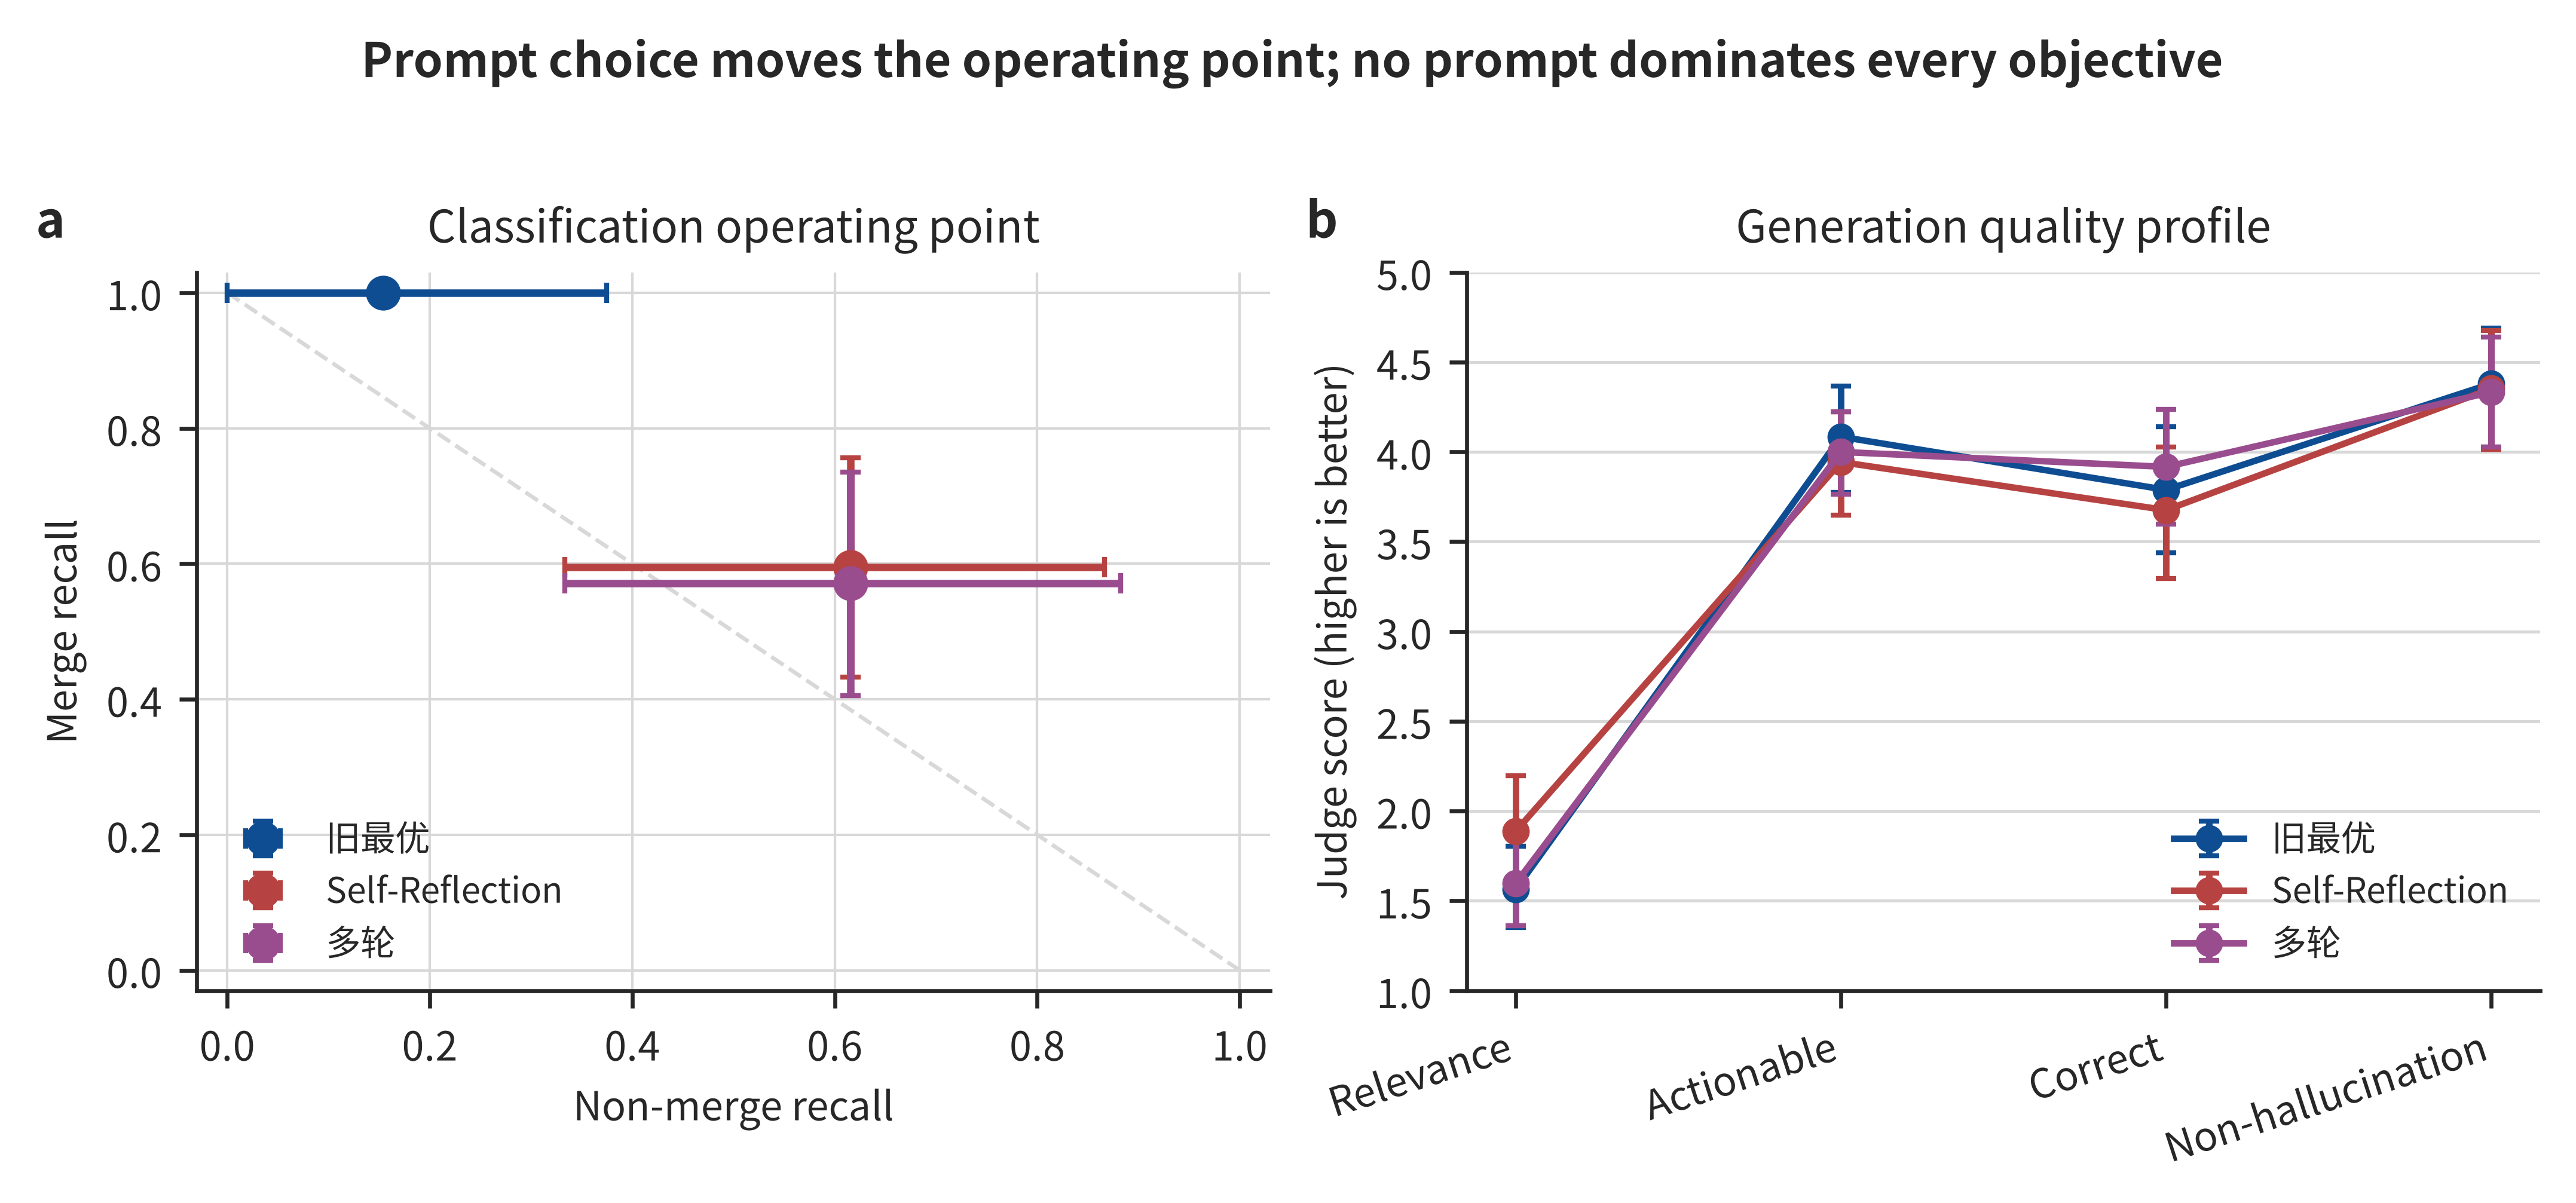
\includegraphics[width=0.98\textwidth]{fig3_prompt_tradeoff.pdf}
\caption{L4 下的 Prompt 性能权衡。\textbf{a}，分类的 non-merge recall 与 merge recall。\textbf{b}，生成任务的四维裁判质量，其中 non-hallucination 定义为 $6-\mathrm{hallucination}$。点为样本统计量，误差线为 95\% bootstrap 置信区间。P5/P6 提高了未合并类召回，并降低了已合并类召回；生成侧各 Prompt 在不同维度取得较高分数。}
\label{fig:prompt-tradeoff}
\end{figure}

生成侧，P5 的 relevance 由 1.563 升至 1.887，correct 从 3.789 降至 3.676，hallucination 从 1.620 升至 1.648。P6 的 correct 最高，为 3.917；其 relevance 为 1.597。各 Prompt 对应不同质量侧重：P5 更关注参考意见中的问题，P3 具有更低时延和更少幻觉，P6 提高了正确性点估计。

\subsection{配对错误转移与作用归因}

逐样本配对分析展示了 P5 的分类变化（图~\ref{fig:error-transition}）。在 13 个 non-merge PR 中，P5 保持 2 个原正确样本，新修复 6 个，仍误判 5 个；在 37 个 merged PR 中，P5 保持正确 22 个，新增 15 个错误拒绝。P5 将模型从接近全判合并的位置移向更保守的工作点。该工作点更适合重视缺陷召回的风险初筛，自动合并场景则需要控制误拒。

\begin{figure}[H]
\centering
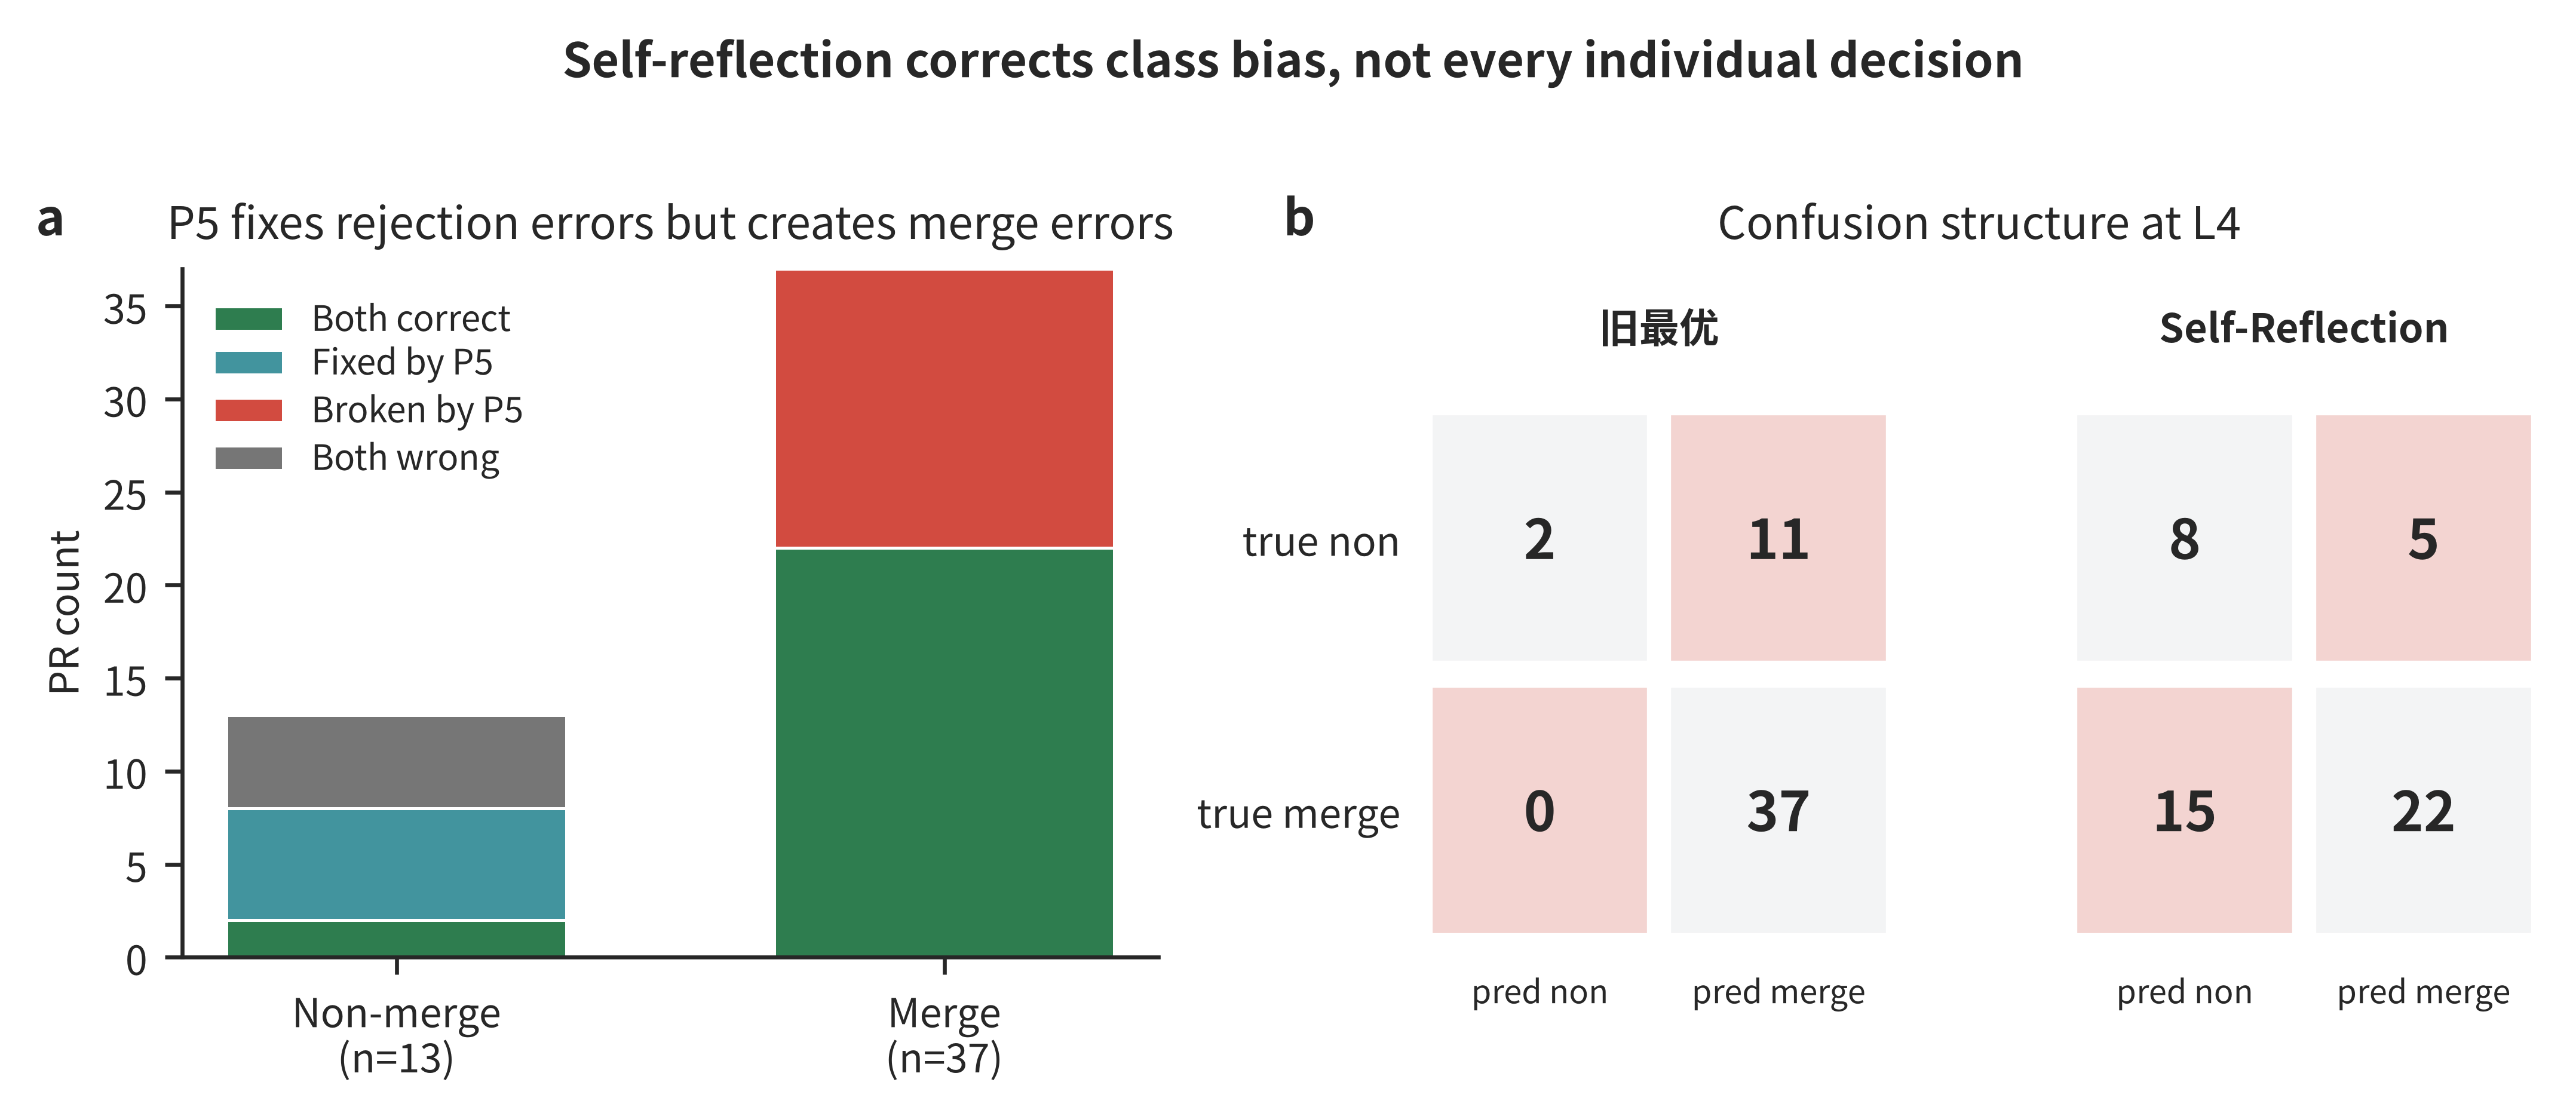
\includegraphics[width=0.98\textwidth]{fig4_error_transitions.pdf}
\caption{P1 到 P5 的分类错误转移。\textbf{a}，50 个 PR 的逐样本配对转移，展示 P5 修复的未合并样本和新增的已合并误拒。\textbf{b}，L4 下两种 Prompt 的混淆结构。配对分析不进行抽样替换，直接反映同一测试集上的决策变化。}
\label{fig:error-transition}
\end{figure}

归因格区分了上下文与 Prompt 的作用。L4$\times$P1 的 balanced accuracy 为 0.577、non-merge recall 为 0.154，深上下文保留了 P1 的合并倾向。L0$\times$P5 的 balanced accuracy 为 0.436、non-merge recall 为 0.385、merge recall 为 0.486，批判性审查在浅层证据下产生较多拒绝。L4$\times$P5 的三项指标分别达到 0.605、0.615 和 0.595。Prompt 控制审查姿态与错误偏好，上下文提供验证缺陷所需的证据。

\subsection{自动生成审查意见样例}

在 \texttt{apache/airflow\#63368} 上，P5 生成的核心意见为：“在 \texttt{\_\_str\_\_} 中使用 \texttt{if detail is not None} 代替 truthiness 检查，以确保空字典或空列表等非 \texttt{None} 但有意义的 detail 也能被附加；同时修复缺失 detail 属性的测试。”人类参考意见同样指出 \texttt{detail} 可能缺失，并强调显式的 \texttt{is not None} 能保留空容器或空字符串等有意义的 falsy 值。裁判给出 relevance=5、actionable=5、correct=5、hallucination=1。

模型依据完整代码与反思 Prompt 定位边界条件，并给出具体修改和测试建议。生成内容与人类意见命中同一缺陷，裁判评分也确认其相关性、正确性和可执行性。该案例展示了 P5 在证据充分时的生成能力。P5 的总体 relevance 均值为 1.887，高质量意见在当前样本中仍不普遍。

\subsection{与实验五及匹配人类代码的比较}

实验六的 L0$\times$P1 分类结果与实验五 C1$\times$P1 完全一致（Accuracy=0.760，merge-F1=0.860），完成了旧基线复现。逐类指标进一步显示，旧 P1 在 L0--L4 的 balanced accuracy 为 0.500--0.583，non-merge recall 为 0--0.167。混淆矩阵揭示了高 merge-F1 背后的多数类偏向，P5 将 L4 non-merge recall 从 0.154 提高至 0.615。生成侧，BLEU 将 L4 排在较高位置，四维裁判则将 L3 排在首位；语义和工程质量指标为开放式审查意见提供了更清晰的区分。

匹配人类对照检验输入方案对不同代码来源的适用性（图~\ref{fig:human-control}）。旧 Prompt 下，AI 与人类分类 balanced accuracy 分别为 0.577 和 0.588，生成 relevance 分别为 1.563 和 1.551；P5 下对应值分别为 0.605/0.478 和 1.887/1.776。各组置信区间明显重叠。P5 提高了 AI 分类的 balanced accuracy，在人类对照上则降低该指标，显示出代码来源与 Prompt 之间的交互。

\begin{figure}[H]
\centering
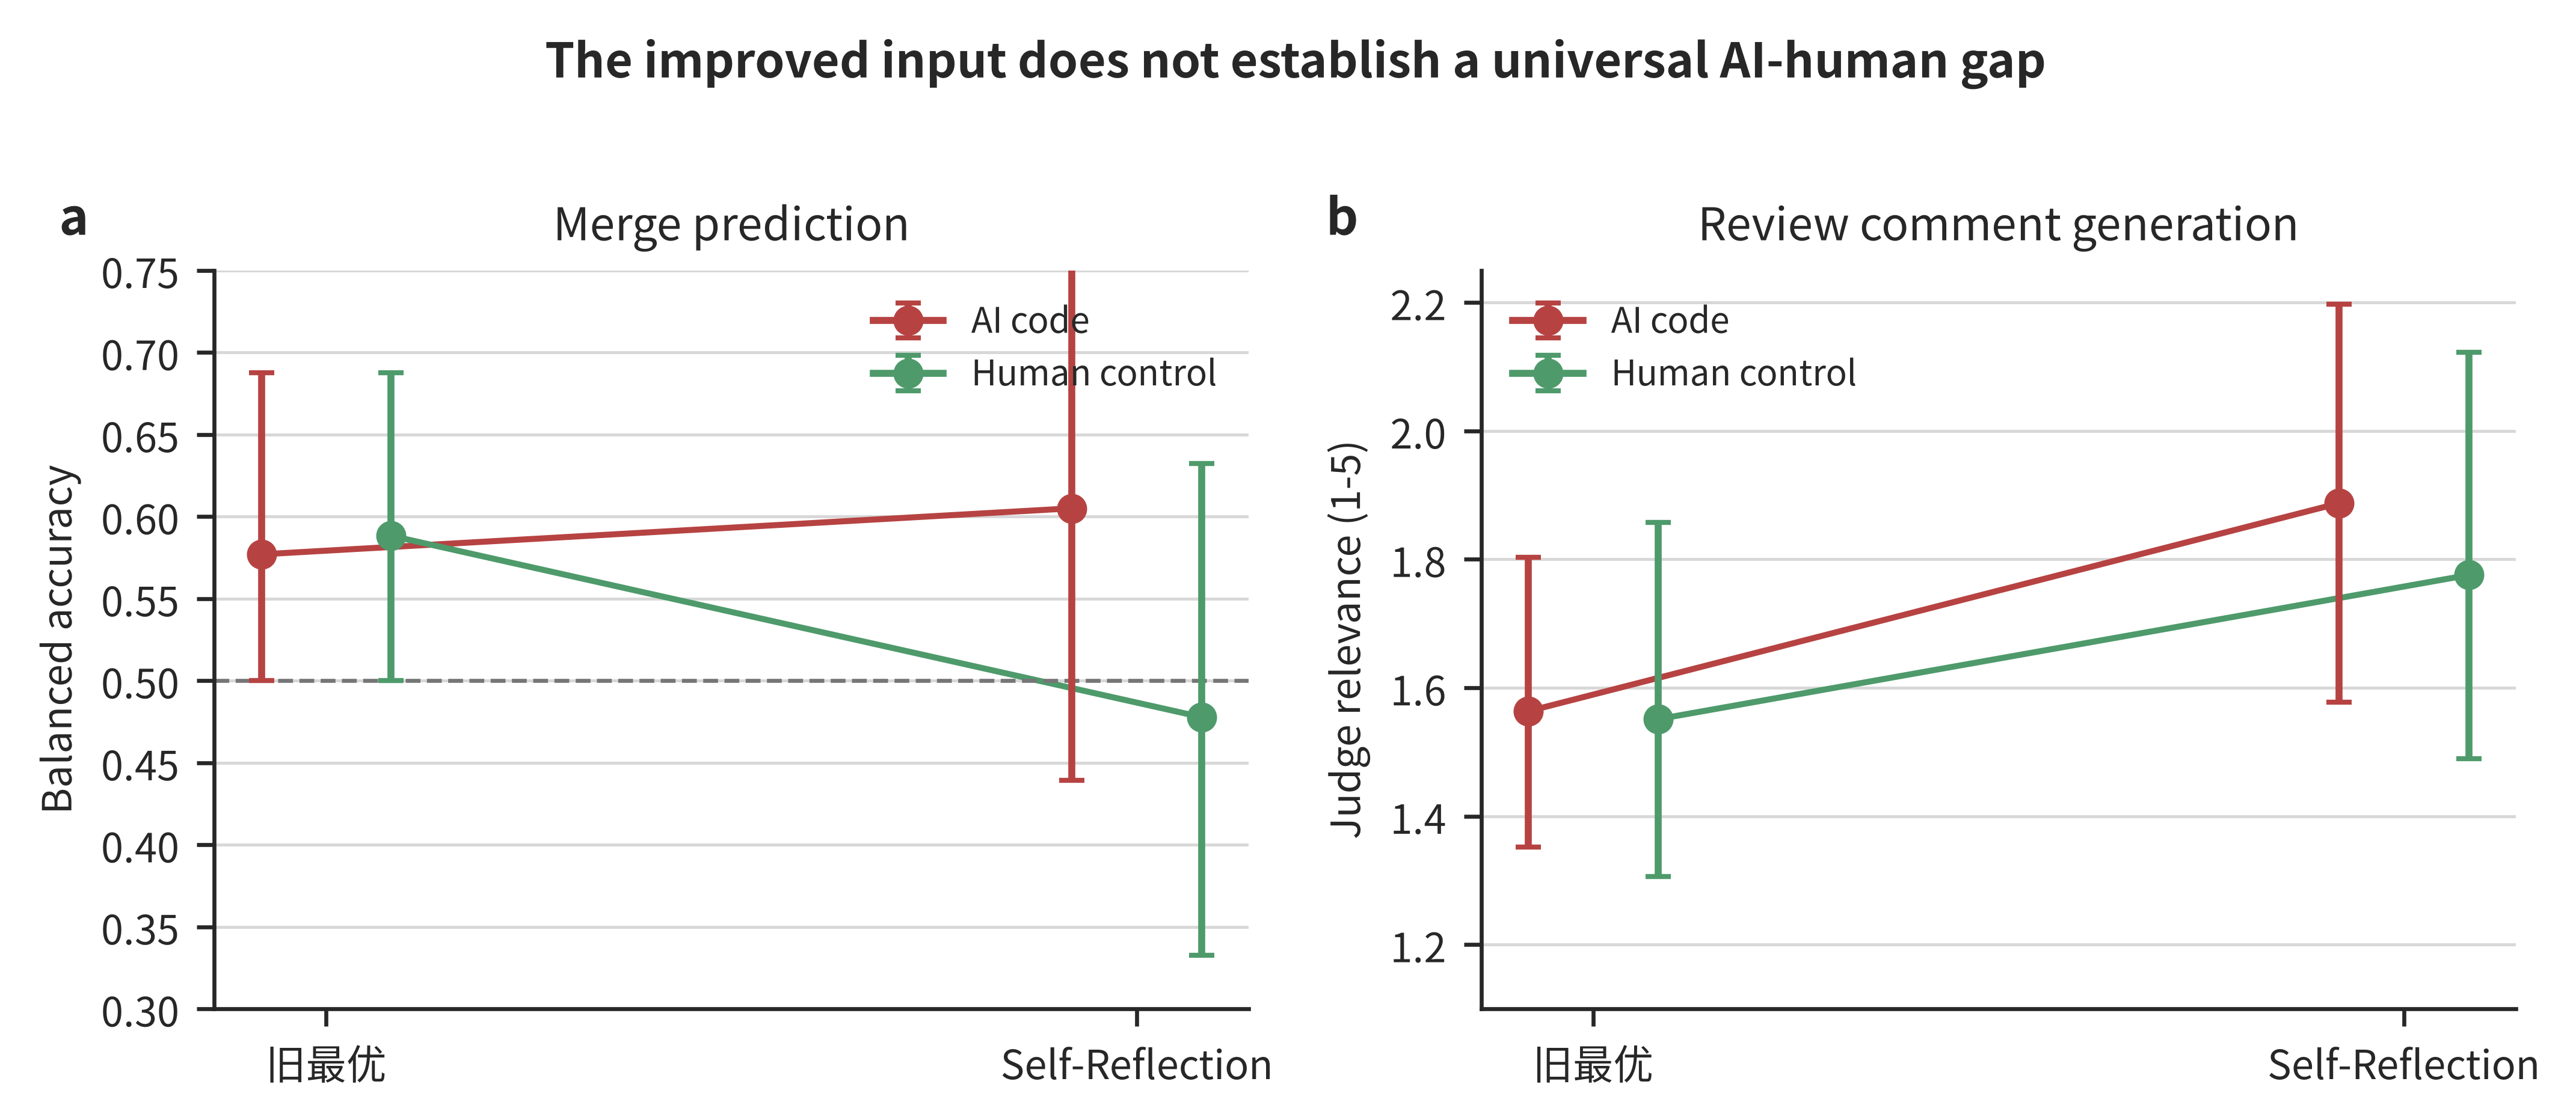
\includegraphics[width=0.98\textwidth]{fig5_human_control.pdf}
\caption{AI 代码与匹配人类对照的关键条件比较。\textbf{a}，Merge Prediction 的 balanced accuracy。\textbf{b}，Review Comment Generation 的 relevance。AI 与人类分类各 $n=50$；生成 AI 原池为 72 个 PR，对照为 50 个 PR。误差线为 95\% bootstrap 置信区间。区间均有明显重叠，且 P5 对两类代码的分类影响方向不同。}
\label{fig:human-control}
\end{figure}

\subsection{质量--成本权衡与下游部署启示}

图~\ref{fig:quality-cost} 联合比较质量与实测时延。分类 P6 平均时延为 42.83~s，是 P1 的 12.27 倍、P5 的 2.70 倍；生成 P6 为 44.42~s，是 P3 的 2.82 倍。P6 的分类 balanced accuracy 低于 P5，生成复合质量与 P3、P5 接近。实验七的交互式 VSCode 插件可使用旧 Prompt 提供低延迟预览，并将 P5 用于高风险 PR 复核。

\begin{figure}[H]
\centering
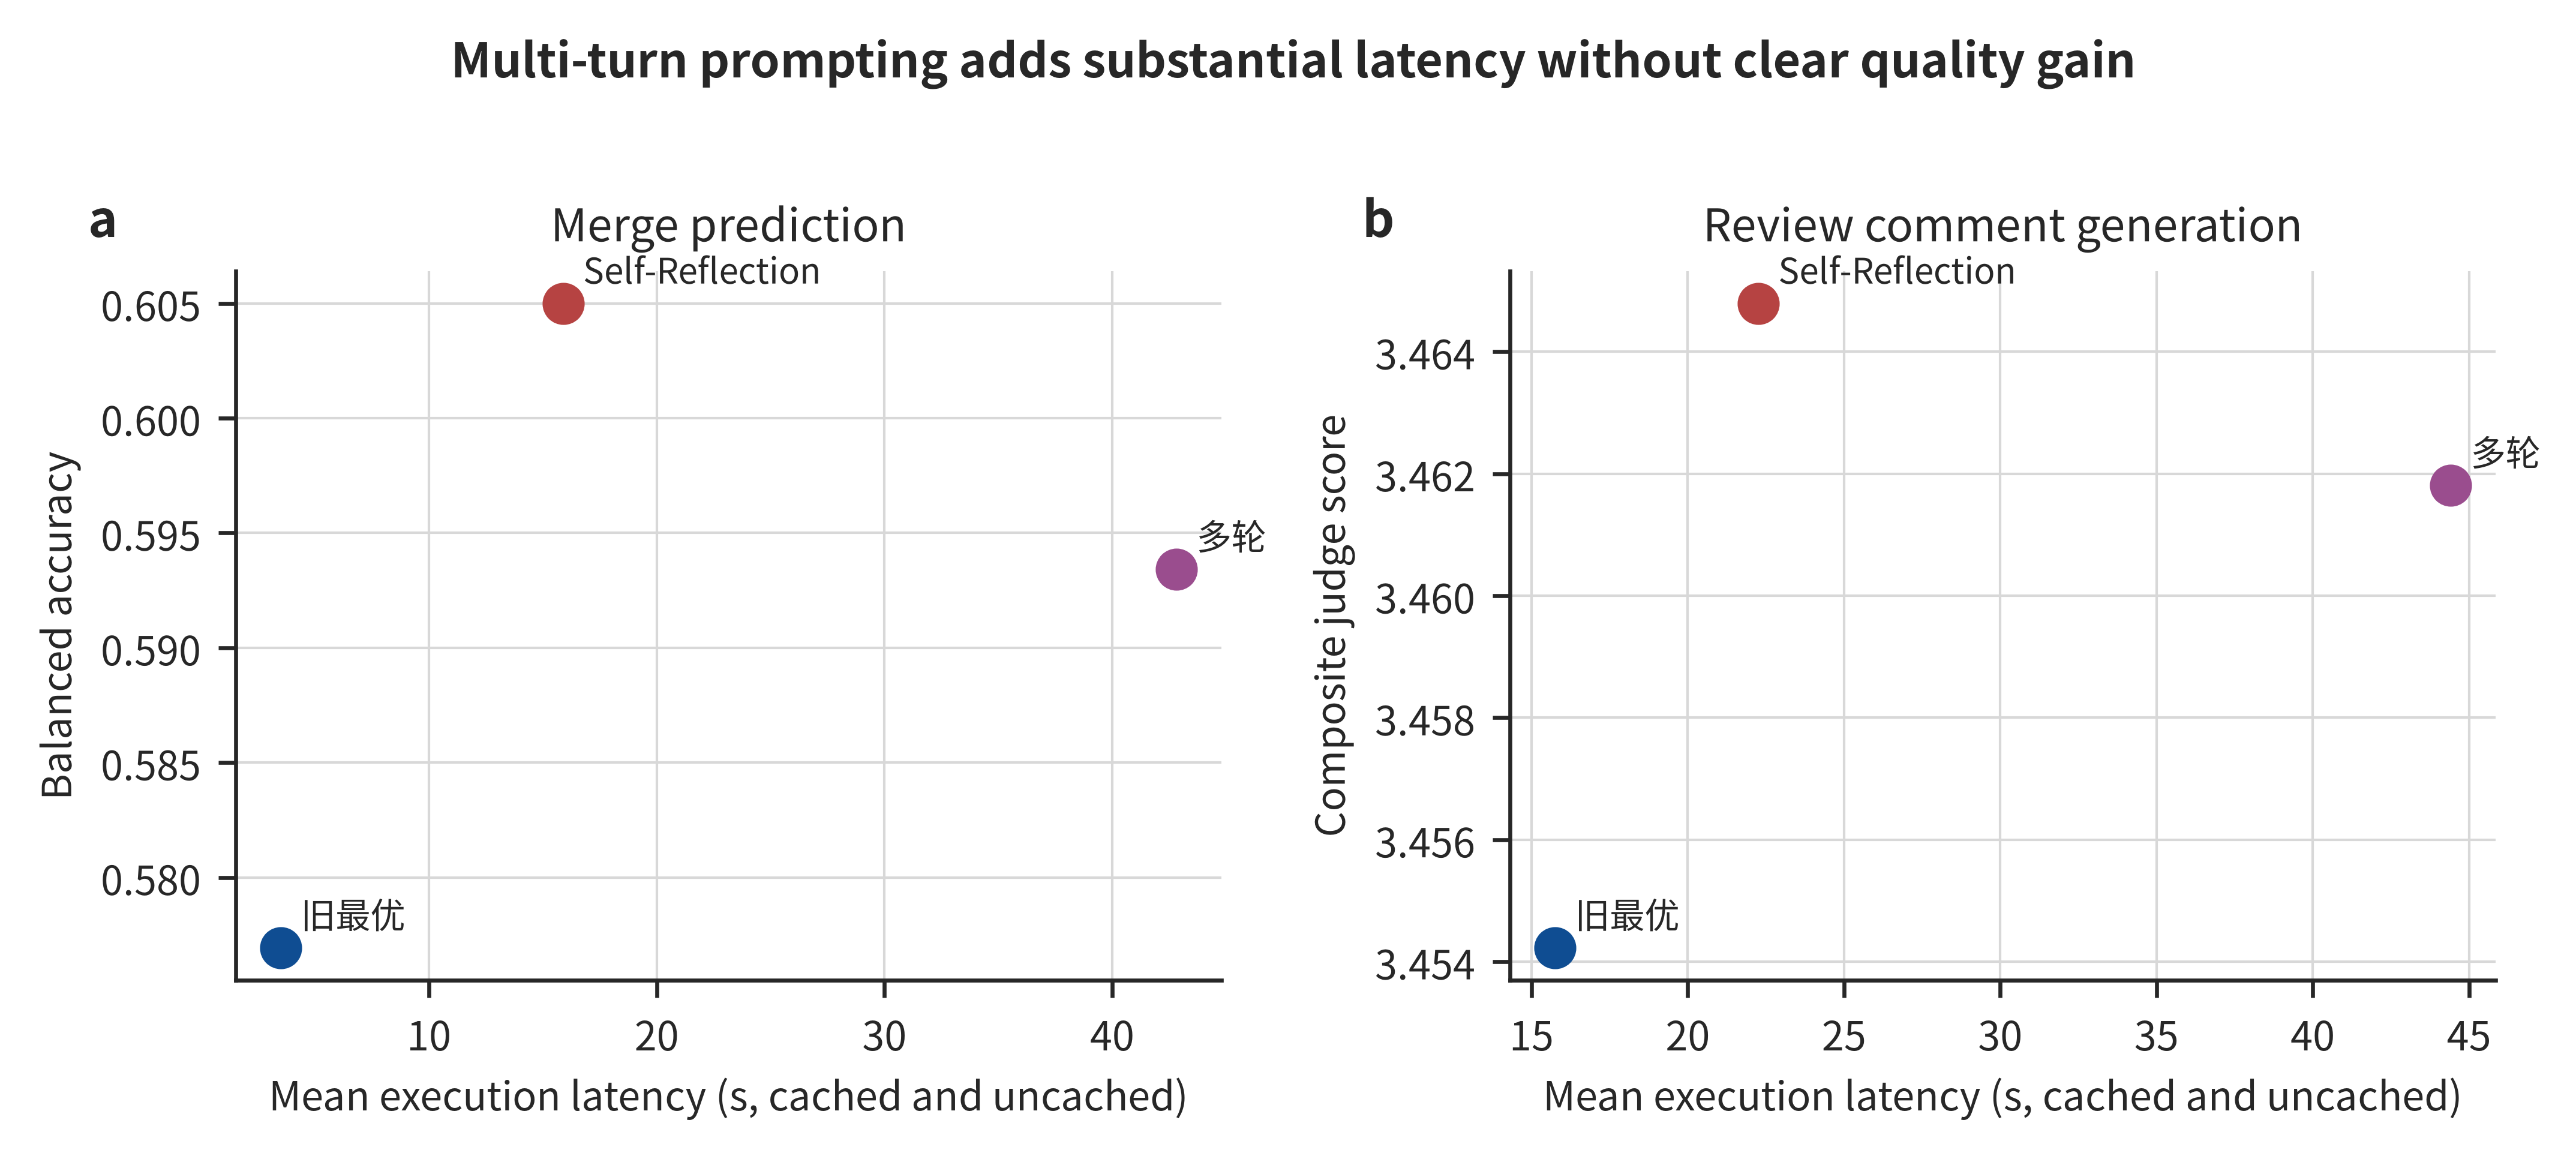
\includegraphics[width=0.98\textwidth]{fig6_quality_cost.pdf}
\caption{Prompt 的质量--成本权衡。横轴为本次实验记录的平均执行时延，纵轴分别为分类 balanced accuracy 和生成复合裁判分。P6 的多轮调用显著增加时延，分类 balanced accuracy 低于 P5，生成复合质量与 P3、P5 接近。}
\label{fig:quality-cost}
\end{figure}

\subsection{结论}

综合上下文阶梯、Prompt 消融、逐样本转移、人类对照和成本分析，本实验得到以下结论：

\begin{enumerate}[label=\arabic*.]
	\item 实验五的高 merge-F1 确实掩盖了近似恒预测“合并”的行为；逐类 Recall、balanced accuracy 和混淆矩阵是评估 AI 合并预测不可缺少的测量工具。
	\item P5 Self-Reflection 将 L4 non-merge recall 从 0.154 提高到 0.615，merge recall 从 1.000 降至 0.595，模型的分类工作点明显向缺陷召回移动。
	\item 完整函数以及 Issue/历史审查取得了更稳定的点估计。上下文质量取决于信息与任务的相关性。
	\item 生成侧 P5 提高 relevance，P3、P5、P6 的复合质量接近。BLEU 与四维裁判给出不同排序，开放式审查意见需要语义和工程价值指标。
	\item P6 的调用成本最高，质量与 P3、P5 接近。实验七可按代码来源和错误成本分级路由，并用精准检索、静态分析、测试和工具调用验证模型提出的阻断性缺陷。
\end{enumerate}

结论的适用范围由当前实验设置限定：分类样本仅含 13 个 non-merge PR，多数组间置信区间重叠；历史 merge outcome 混合代码质量与项目流程因素；生成评价使用单条参考意见，裁判模型与执行模型属于同一模型系列；L4 实现的是轻量词法检索。现有证据表明，高相关上下文与批判性 Prompt 可以按任务目标改变 AI 代码审查行为，跨仓库推广和更精确的仓库级检索仍需独立验证。

}

%========================
% 问题总结
%========================

\experimentproblems{

\subsection*{4.1 深层上下文的获取与复现}

L2--L4 需要根据 PR 的 base SHA 和 head SHA 获取完整文件、Issue、历史审查意见及仓库检索结果。直接重复请求 GitHub API 容易受到网络波动和访问频率限制，也会使不同运行之间的输入难以保持一致。为此，实验为文件、Issue 和检索结果建立了落盘缓存，并采用固定的内容排序、字符预算和截断规则。重跑时优先读取缓存，从而减少重复请求并保证同一 PR 在相同条件下获得一致输入。

\subsection*{4.2 分类指标受类别不平衡影响}

AI 分类样本中已合并 PR 占 74\%，Accuracy 和 merge-F1 容易受多数类预测影响。实验补充 non-merge 与 merge 两类的 Precision、Recall、F1、混淆矩阵及 balanced accuracy，并用 non-merge recall 检查 P5 对合并偏向的影响。完整指标显示，P5 提高了未合并类召回，也增加了已合并 PR 的误拒。

\subsection*{4.3 开放式审查意见难以用词面指标评价}

一处代码修改可能对应多种合理审查意见，不同表达会降低生成文本与单条参考意见的词面重合。实验保留 BLEU 和 ROUGE 用于实验五对比，并引入裁判模型，从相关性、可操作性、正确性和幻觉四个维度评价生成结果，再结合具体案例核对评分。该评价提供了词面重合之外的质量信息。

}

%========================
% 实验体会
%========================

\experimentexperience{

\subsection*{5.1 对软件工程上下文的认识}

本实验使我认识到，上下文的价值取决于其与审查任务的相关性。完整函数以及 Issue、历史审查意见补充了局部 Diff 缺少的实现和需求信息，仓库级词法片段的收益则受检索质量影响。分层消融能够识别每类工程证据的实际作用。

\subsection*{5.2 对 Prompt 优化的认识}

Prompt 会同时影响输出结构和审查姿态。P5 引导模型先寻找阻断性缺陷，提高了 non-merge recall，也造成更多误拒。Prompt 选择需要对应任务的错误成本：高风险审查重视缺陷召回，自动合并重视对正常 PR 的准确放行。

\subsection*{5.3 对实验评价与工程应用的认识}

代码审查系统需要联合评价逐类指标、混淆矩阵、生成质量和推理成本。实验中的多轮推理显著增加了时延，质量变化较小。后续 VSCode 插件可以按风险分级使用不同 Prompt，并将模型意见与测试、静态分析等可验证工程证据结合。

}

%========================
% 教师评语
%========================

\teachercomment

\end{document}